\chapter{Arquitectura del \textit{pipeline}}
\label{cap:arquitecturaPipeline}

El objetivo final de este trabajo se resume en montar un \textit{pipeline} que permita jugar a un videojuego con la mente. Este capítulo explica precisamente el \textit{pipeline} diseñado para conseguirlo.

La implementación del \textit{pipeline} en tiempo real se divide en dos fases inicialmente. Siendo la primera el entrenamiento del modelo y la obtención de la matriz de alineamiento euclideo y, la segunda, el funcionamiento en tiempo real del sistema. 

\begin{itemize}
	\item \textbf{Fase 1: Obtención de datos para el entrenamiento del modelo.} En esta fase se recopilan datos (basándose en el \hyperref[cap:protocoloAdquisicion]{protocolo de adquisición} más adelante explicado) necesarios para el \textit{fine-tuning} del modelo y la generación de la matriz de alineamiento euclideo usada para normalización. Se desarrollaron dos procesos independientes: uno encargado de visualizar la interfaz gráfica del experimento, indicando de forma visual al usuario la acción de imaginación motora que debía realizar en cada instante, y otro responsable de recibir los datos procedentes del dispositivo EEG.
	
	\begin{enumerate}
		\item \textbf{Proceso 0:} encargado de visualizar la interfaz gráfica del experimento, indicando de forma visual al usuario la acción de imaginación motora que debe realizar en cada instante.
		\item \textbf{Proceso 1:} este actúa como proceso principal del sistema. Es responsable de crear el proceso anteriormente mencionado, gestionar la adquisición de datos EEG, realizar las anotaciones correspondientes sobre la grabación e indicar al \textbf{proceso 0} dinámicamente las señales visuales que deben presentarse durante el experimento.
	\end{enumerate}

	Ambos procesos se comunican mediante una tubería unidireccional, a través de la cual el proceso coordinador envía instrucciones al proceso encargado de la interfaz gráfica indicando qué símbolos deben mostrarse al usuario en cada momento.

	Una vez finalizada la recolección de datos, se preprocesan los datos en el \textbf{proceso 1}, se calcula la matriz de alineamiento euclideo y se realiza \textit{fine-tuning} en el modelo. Tras esto, se inicia la \textbf{fase 2}. 

	\item \textbf{Fase 2: Funcionamiento en tiempo real.} Esta describe el funcionamiento en tiempo real por completo. Desde la obtención de datos, pasando por el procesamiento de los mismos, hasta la salida producida. Para el \textit{pipeline} en tiempo real se decidió emplear 4 procesos representados en el diagrama \ref{fig:pipelineTR}.
	
	\begin{enumerate}
		\item \textbf{Proceso 1: Recolector de datos y coordinador.} El mismo proceso encargado de recibir los datos del dispositivo EEG es reutilizado para esta fase. Sus responsabilidades son crear los demás procesos y recoger continuamente datos del dispositivo EEG y retransmitirlos inmediatamente.
		\item \textbf{Proceso 2: \hyperref[cap:tratamientoDatos]{Tratamiento de los datos} y \hyperref[cap:modelo]{modelo}.} A nivel de implementación y cálculos, es el más grande de todos. Trata los datos recibidos y aplica inferencia sobre el modelo para clasificarlos en tiempo real.
		
		Para ello, dispone de un \textit{buffer} circular capaz de almacenar continuamente los datos retransmitidos por el dispositivo EEG en los últimos 15 segundos. A pesar de que las predicciones posteriores se realizan utilizando únicamente ventanas temporales de 4 segundos, el uso de un \textit{buffer} más amplio permite mejorar la aplicación de \hyperref[subsec:FiltradoFrecuencia]{filtros de bajas frecuencias}. 
		
		Este proceso se divide internamente a su vez en dos hilos de ejecución: 

		\begin{enumerate}
			\item \textbf{El primero} se encarga de recibir los datos procedentes de la tubería de comunicación y almacenarlos en el \textit{buffer} circular, evitando así posibles desbordamientos del pipe debido a la falta de frecuencia de adquisición de datos.
			
			Al invocar la función \texttt{getData} del \textit{buffer} circular, los \hyperref[subsec:FiltradoFrecuencia]{filtros de frecuencia} se aplican sobre la ventana completa de 15 segundos dentro de este hilo. Posteriormente, se extraen únicamente los últimos 4 segundos filtrados, que constituyen el \textit{trial} utilizado para la predicción, y se envían al siguiente.
 
			\item \textbf{El segundo} es responsable de generar predicciones periódicas a partir de los datos almacenados en el \textit{buffer}, alcanzando una frecuencia aproximada de 6,6 predicciones por segundo.
			
			Este recibe el \textit{trial} y le aplica, en primer lugar, el alineamiento euclídeo haciendo uso de la matriz calculada previamente. A continuación, realiza la \hyperref[sec:interpolación_espacial]{interpolación espacial} con el objetivo de adaptar el número y disposición de canales EEG a la configuración esperada por el modelo.

			Finalmente, el \textit{trial} resultante es clasificado por el modelo, enviándose posteriormente la predicción resultante al siguiente módulo.

		\end{enumerate}
		
		Una vez obtenido el 
		\item \textbf{Proceso 3: \hyperref[sec:filtros_decision]{Intérprete del flujo de predicciones}.} Gestiona el flujo constante de predicciones que recibe del anterior bloque, las procesa y las suaviza haciendo uso de \hyperref[sec:filtros_decision]{filtros de decisión} para simplificar su utilización en el siguiente módulo.
		
		\item \textbf{Proceso 4: \hyperref[sec:filtros_ayuda]{Filtro de ayuda} y \hyperref[cap:juegosPropuestos]{juego} a ejecutar.} Este último es responsable de llevar toda la lógica del juego/\textit{benchmark} que se quiera ejecutar y de decidir qué acción tomar en cada momento, basándose en las predicciones recibidas y el estado del juego en cada instante. 

		Este proceso se diseñó para ser completamente independiente, permitiendo así modularidad y una mayor facilidad de integración en el \textit{pipeline} con diferentes juegos, además de ser una alternativa más estable y compartimentada tratando de aliviar la carga del \textbf{proceso 3}.

		\end{enumerate}

\end{itemize}

\begin{figure}[h]
	\centering
	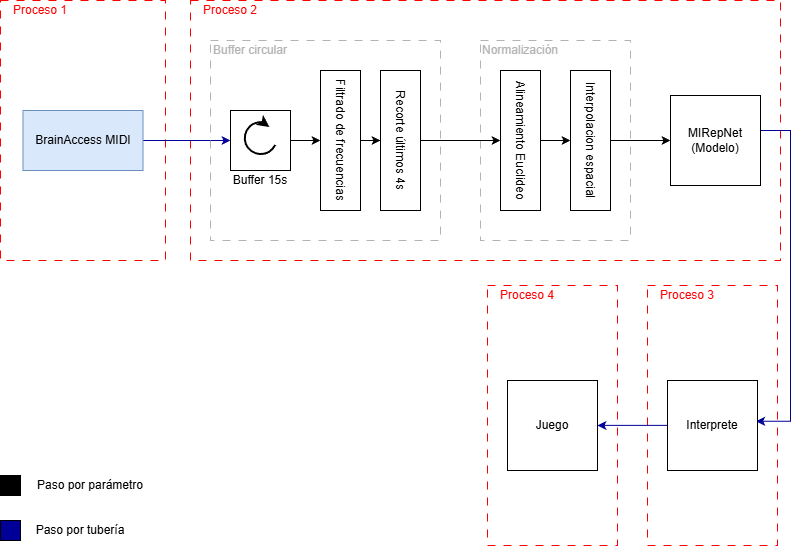
\includegraphics[width=\textwidth]{Imagenes/Bitmap/Pipeline_TR}
	\caption{Diagrama de la arquitectura del \textit{pipeline} en tiempo real.}
	\label{fig:pipelineTR}
\end{figure}

Esta separación en procesos independientes resultó tanto necesaria como beneficioso en ambas fases debido a: evitar posibles limitaciones de concurrencia entre las librerías utilizadas, importancia de gestionar correctamente los recursos del sistema, reducción de latencias, modularización que permita cambios y adaptaciones. 

Por un lado, la librería del dispositivo BrainAccess inicia internamente hilos de ejecución para la adquisición de datos EEG, mientras que la librería empleada para mostrar la interfaz gráfica también gestiona su propia concurrencia de forma interna. Al intentar ejecutar ambas funcionalidades dentro de un único hilo de ejecución, se producían bloqueos y fallos de funcionamiento, por lo que fue imprescindible desacoplar ambas tareas mediante \textit{multiprocessing}.

Por otro lado, la separación de la última funcionalidad en un bloque independiente evita que elementos externos al \textit{pipeline} BCI, como una interfaz gráfica o la lógica del videojuego, compitan por recursos computancionales con el sistema de adquisición y clasificación EEG. Y así no introduzcan latencias adicionales o fallos inesperados.

Además, permite aprovechar la concurrencia para reducir la latencia global del sistema.

También facilita los cambios modulares: favoreciendo variar el \hyperref[cap:modelo]{modelo} usado, escoger entre los distintos \hyperref[sec:filtros_decision]{filtros de decisión}, probar distintos \hyperref[cap:juegosPropuestos]{juegos}\dots

Por último, esta arquitectura deja abierta la posibilidad de distribuir los diferentes procesos en máquinas independientes (en lugar de procesos) sustituyendo las tuberías locales por sockets TCP. Aunque esta funcionalidad distribuida no ha sido implementada en el presente trabajo, permitiría ejecutar el pipeline de inferencia en servidores externos con capacidad GPU, facilitando así el uso del dispositivo desde equipos con recursos computacionales limitados.
